\documentclass[]{article}
\usepackage[utf8]{inputenc}
\usepackage[danish,english]{babel}
\usepackage{graphicx}
\usepackage[usenames]{xcolor}
\usepackage{times}
\usepackage{listings}
\usepackage{textcomp}
\usepackage{hyperref}
\usepackage{textpos}
\usepackage{pgfgantt}
\usepackage{lscape}
\usepackage{indentfirst}
\usepackage{tikz}
\usepackage{pgfplots}
\usepackage{ifthen}
\usepackage{float}
\usepackage{pict2e}
\usepackage[export]{adjustbox}
\pgfplotsset{compat=1.13}
\usepackage{siunitx}
\usepackage{tabularx}

% adjustment to page format
\marginparwidth=0pt
\oddsidemargin=0pt
%\evensidemargin=0pt
\marginparsep=0pt
%\topmargin=-15 mm
\textwidth=168 mm
\textheight=210 mm
\parskip 0.27 em
\parindent=0pt
%\leftmargin=1cm
\pagenumbering{arabic}
% Define DTU color
\definecolor{dtured}{RGB}{153,0,0}
\title{Projektplan}

\begin{document}
% formel header
\thispagestyle{empty}
\vspace*{-1.9cm}
\begin{textblock*}{18cm}[0,0](0cm,-2cm) %
  \noindent
  
\includegraphics[width=4.5cm,valign=t]{documentation/resources/tex_dtu_elektro_a.pdf}
  \hspace*{10.6cm}
  
\includegraphics[width=1.5cm,valign=t]{documentation/resources/tex_dtu_logo.pdf}
\end{textblock*}
\begin{textblock*}{19.0cm}(0cm,-2.5cm) %
\begin{center}
  {\color{dtured}\large31015 Introductory project}\\
  \normalsize
  s186083 Tjark Petersen\\
  s194006 Steffan Martin Kunoy\\
  s194027 Victor Alexander Hansen\\
\end{center}
\end{textblock*}
% rød streg
\vspace{1mm}
{\hspace*{-0.1cm}
\color{dtured}\noindent \rule{16.8cm}{5pt}}

 
\begin{table}[H]
     \centering
     \begin{tabularx}{\textwidth}{|X|X|X|}
     \hline
          DTU Electro&Spring 2021 & Group: 7, ID: MEK2 \\\hline
          Course 31015 & Title & Group members \\\hline
          Introductory project - Electrotechnology & ROAST Telemetry & \begin{tabular}{l} s186083 Tjark Petersen\\s194006 Steffan Martin Kunoy\\s194027 Victor Alexander Hansen \end{tabular}\\\hline
          Document:& Project plan & 4 pages\\\hline 
          Version/Status: & 1. edition &\today\\\hline
     \end{tabularx}
 \end{table}
 
\section{Problem introduction}

This project will concern a telemetry module for use by the DTU Roadrunners Solar Team (ROAST). In 2023 ROAST is set to participate in the Bridgestone World Solar Challenge, a race spanning 3000 km across Australia \cite{wsc}. The solar car must be able to drive 3 stretches of 1200 km without recharging. Thus, solar power will be the main energy source during the race. \\
%Dette projekt vil omhandle et telemetri modul som skal indgå i DTU Roadrunners Solar Team (ROAST). I 2023 deltager ROAST i Bridgestone World Solar Challenge, som er et løb på over 3000 km tværs gennem Australien \cite{wsc}. Solbilen skal køre en distance på 3 x 1200km, hvor bilen ikke har mulighed for at oplade. Den primære energikilde for bilen under løbet er derfor solenergi.\\
\\
Throughout the race the solar car will be monitored by a support car, which can monitor the car's conditions and issue commands. This is a crucial function as the solar car will be navigating Australia's busy highways, where the heat and tire pressure may cause a detriment to the vehicle. The support car will therefore be able to analyze and react to the data stream being transmitted from the solar car, even when the driver is preoccupied by driving the car and navigating traffic. \\
%I løbet vil solbilen være ledsaget af en følgebil, som skal overvåge solbilens driftstatus og sende kommandoer til solbilen. Dette er en yderst vigtig opgave, da bilerne skal køre tværs gennem Australien i offentlig trafik, hvor alt fra varme til dæktryk udfordrer solbilen. Følgebilen vil derfor have mulighed for at analysere og reagere på data fra solbilen, hvis køreren i solbilen er optaget af trafik og betjening af solbilen.
\\
The main function of the telemetry module is to read data from the solar car's onboard CAN (Controller Area Network) bus and transmit it via an RF-transceiver to the support car, while simultaneosly logging data locally in a "black box" memory chip. The support car is equipped with a similar module such that the support crew can react to the data manually or automatically by sending commands back to the CAN bus. As a consequence, the telemetry module plays a vital role in the communication between both vehicles, considering the distance between them may be up to 1 km depending on traffic conditions. 
%Telemetri modulets opgave er at aflæse sensordata fra solbilens CAN (Controller Area Network) bus og sende dataen via en RF-transceiver til følgebilen såvel som at logge dataen lokalt i et "black box" hukommelseschip. Et lignende modul skal også være til stede i følgebilen, så følgebilen omvendt kan reagere på denne data, enten automatisk eller ved menneskelig ageren, og sende kommandoer tilbage til solbilens CAN bus. Telemetri modulet spiller derfor en afgørende rolle, da man også skal tage højde for at afstanden mellem solbil og følgebil kan være op til 1 km alt afhængig af trafikforholdene.

\section{Problem description}
Remote sensing of data from the solar car will give the ROAST team a competitive advantage as the support vehicle will take on a more active role in controlling and optimising the car's performance. This will ease the burden on the driver and engage a large part of the supporting crew. For these reasons we have chosen to focus our project on the following points:   
%Fjernmåling af data fra solbilen vil give ROAST en fordel i og med at support bilen kan indtage en mere aktiv rolle i styring og optimering af bilen. Det letter derfor på kørerens arbejdsbyrde, og fordeler ansvaret for hele ROAST-support holdet. Af denne grund vil vi afgrænse projektet på følgende punkter: 
\begin{itemize}
    \item How can we design a module that can read and write sensor data and commands from a CAN bus network? 
    %\item Hvordan kan vi lave et modul der kan læse, sende og modtage sensor data og kommandoer i CAN bus netværket?
    \item How can CAN data be transmitted over a distance of up to one kilometer? 
    %\item Hvordan kan CAN data overføres trådløst i en afstand på en kilometer?
    \item How does the support-car module process data upon receiving it from the solar car?
    %\item Hvordan skal data behandles ved modtagelse i følgebilen?
    \item What is the best method for storing data locally (black box) while being accesible at a later time? 
    %\item Hvordan kan data bedst gemmes lokalt (black box) og udlæses på et senere tidspunkt?
\end{itemize}

\section{Afgrænsning}
Vi har i vores gruppe diskuteret flere forskellige umiddelbare løsningsformer for projektets produkt, heriblandt at lave en løsning på et PCB board, eller en løsning på et Teensy board/FPGA board. Vi har valgt at afgrænse os til at se på Teensy og FPGA løsninger, og ikke PCB boards. Dette skyldes at det hardware design vi kommer frem til som produkt kan redigeres mere fleksibelt undervejs på et Teensy og FPGA board, fremfor et PCB board som er mere special designet til formålet.\\
\\
Det skal dog siges at vi forventer at et PCB board design ville være mindre strømkrævende end de løsninger vi ser på, men vi har i dette projekt valgt at prioritere et godt design over strømbesparelse, siden der formentlig er tale om forskel i størrelsesorden af nogen tiende af mA.
\section{Target audience}
The target audience for our project is the DTU ROAST team, who will integrate the telemetry module in the solar car and support vehicle. Subsequently, the car is set to enter the 2023 Bridgestone World Solar Challenge.

\section{Problem solution}
\begin{enumerate}
    \item Preliminary design of telemetry module in block diagram form. Establish specifications and requirements for the final product. 
    %\item Foreløbigt design af telemetrimodulet som blokdiagram. Fastslå specifikationer og krav til løsningen. 
    \item Select components for preliminary design. Ordering components not available from DTU. 
    %\item Valg af komponenter til det indledende design. Bestilling af komponenter som ikke kan fremskaffes på DTU. 
    \item Prototyping telemetry module on two breadboards. Write code to test limited functionality. 
    %\item Første prototype af telemetrimodul på breadboard. Skrive kode til at teste begrænset funktionalitet. 
    \item Improve on prototype. Order new components if needed. Optimize code and write more extensive tests. 
    %\item Foreslå forbedringer til første prototype. evt. bestille nye komponenter. Optimer kode og design mere omfattende tests.
    \item Improved prototype of telemetry module on breadboard. Repeat Steps 3. and 4. until fundamental requirements in Step 1. are satisfied. 
    %\item Anden prototype af telemetrimodul på breadboard. Gentag 3. og 4. indtil grundlæggende krav i 1. er opfyldt. 
    \item Develop more permanent solution, i.e. compact, soldered and configurable. Complete tests in Step 5.
    %\item Udvikle mere færdig løsning, dvs. kompakt, loddet og programmerbar. Gennemfør tests som i 5.
    \item Design GUI for interaction with PC. Test with USB connection to support-car module. Remote control via PC. 
    %\item Design af GUI til interaktion med PC. Test med USB forbindelse til support-bil modul. Styring via PC.  
    \item Present solution to DTU ROAST team. Discuss improvements and additional features. 
    %\item Præsenter løsning for DTU ROAST holdet. Diskuter forbedringer og features. 
    \item Integrate telemetry module with solar car. Ongoing testing of solution. Feedback and evaluate project. 
    %\item Integration med solbil, løbende tests og evaluering af projekt. 
\end{enumerate}
\section{Resources}
\begin{itemize}
    \item 1x Teensy 4.0 development board
    \item 1x Teensy 4.1 development board
    \item 2x nRF24L01 + PA/LNA Wireless Transceiver with antenna
    \item 1x Micro SD memory card
    \item 1x MCP2551 CAN Transceiver w/ breakout board
\end{itemize}
\newpage


\begin{landscape}
\section{Activity Plan}
\hspace{1.5cm}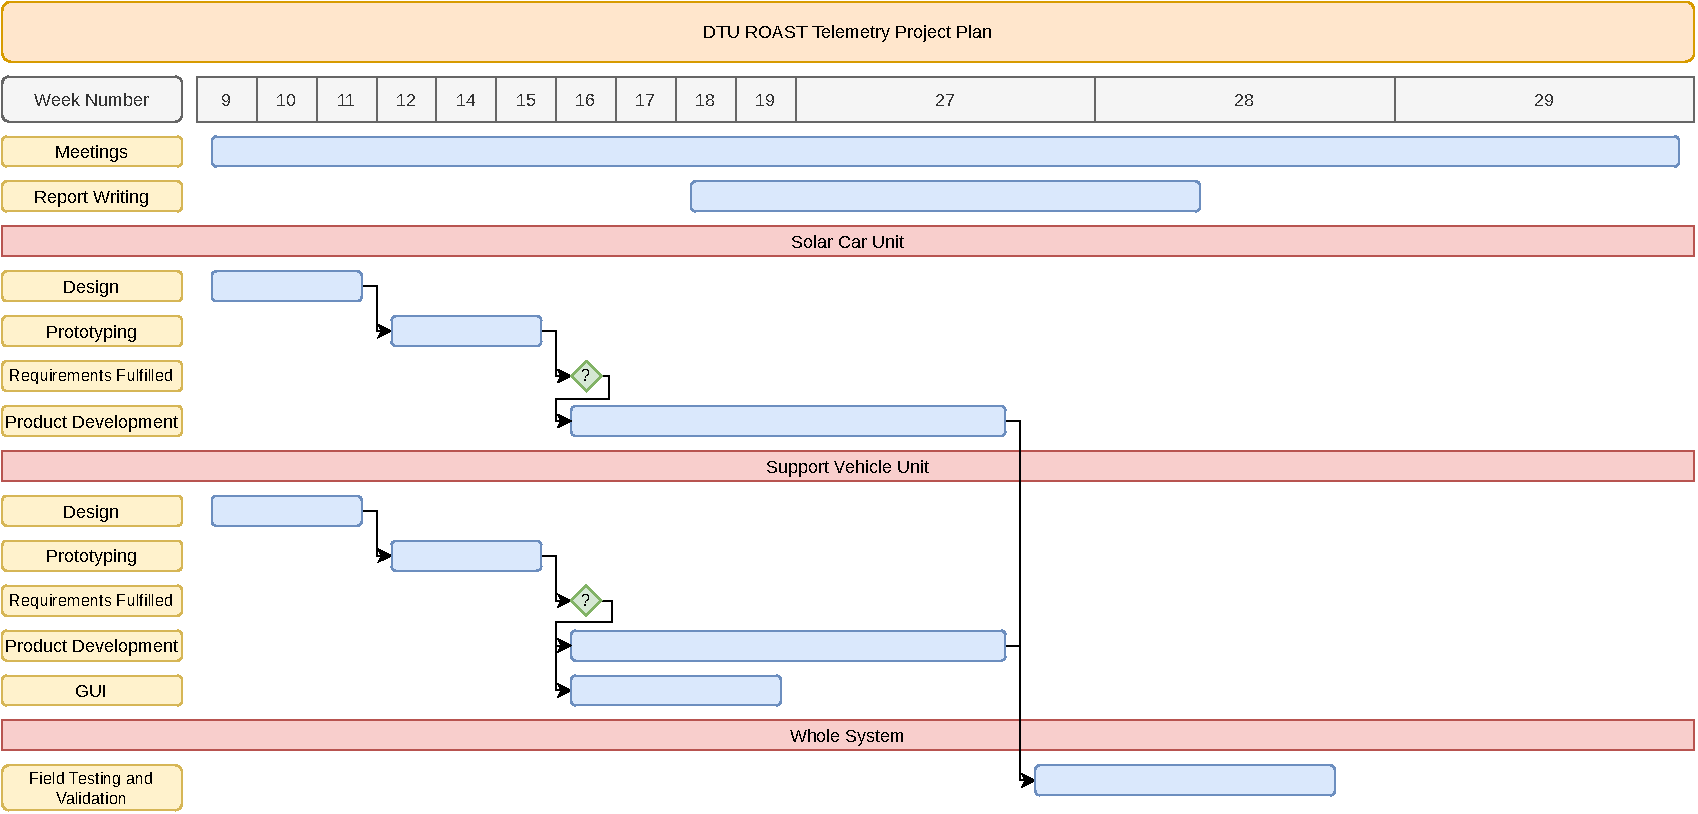
\includegraphics[width=1.35\textwidth]{documentation/images/projectPlan.pdf}
\end{landscape}

\newpage
Meetings:\\
We will have a weekly meeting with both the project coordinator Christian Kampp Kruuse and our advisor Martin Schoeberl at Friday.
Report writing:\\

\section{References}
\begingroup
\renewcommand{\section}[2]{}%
%\renewcommand{\chapter}[2]{}% for other classes
\begin{thebibliography}{}
\bibitem{wsc}
Bridgestone World Solar Challenge, 
URL: https://worldsolarchallenge.org/
\end{thebibliography}
\endgroup
\section{Green challenge?}


\end{document}